\documentclass[a4paper,czech]{article}
\usepackage[T1]{fontenc}
\usepackage[utf8]{inputenc}
\usepackage[czech]{babel}

\usepackage{anysize}
\usepackage{geometry}
%\geometry{a4paper, portrait, margin=2.5cm}

\usepackage{graphicx} % Required for the inclusion of images
\usepackage{amsmath} % Required for some math elements 
\usepackage{fancyhdr} %na headers
\usepackage{multirow}
\usepackage{caption}
\usepackage[colorlinks=false,unicode=true]{hyperref}
\usepackage{indentfirst}
\usepackage{tikz}
\graphicspath{ {images/} }

%\setlist[enumerate]{label*=\arabic*.}
%\setlength\parindent{0pt} % Removes all indentation from paragraphs

\renewcommand\familydefault{\sfdefault}
%\renewcommand{\sectionmark}[1]{\uppercase{\markboth{}{\emph{~#1}}}}
%\renewcommand{\subsectionmark}[1]{}% Remove \subsection from header
\def\tableautorefname{tab.}
\def\figureautorefname{obr.}
\def\sectionautorefname{kap.}
\def\equationautorefname{rovn.}
\def\subsectionautorefname{podkap.}

\begin{document}

\LARGE{\textbf{Otázky na TBK 2018}}
\newpage
\section{Úvod}
\subsection{\textbf{Vyjmenujte alespoň 5 příkladů běžně používaných bezdrátových komunikačních systémů. Najděte k nim pracovní frekvenční pásma.}}

\section{Systémy}
\subsection{\textbf{Nakreslete blokové schéma RX s 2-násobným směšováním a popište funkci.}}
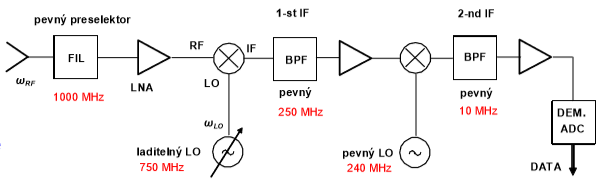
\includegraphics{images/rx_2_nasobny.png}
\begin{itemize}
	\item Používá se vysoká frekvence 1. IF filtru $\omega_IF1$
	\item Zrcadlové pásmo je potom vzdálené a dá se dobře filtrovat, lze použít jednoduchý filtr na fixní frekvenci
	\item Další zpracování na vysoké frekvenci $\omega_IF1$ je neefektivní (horší parametry demodulátoru, vyšší nároky a ADC, ...) a proto se používá 2. přídavný směšovací stupeň.
\end{itemize}
\subsection{\textbf{Nakreslete blokové schéma přijímače s přímou konverzí do základního pásma. Jaké jsou výhody a nevýhody této struktury.}}
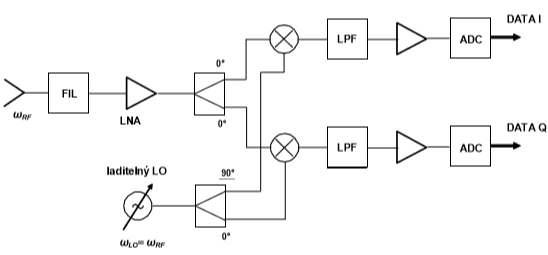
\includegraphics{images/tx_priama_konv.png}
\begin{itemize}
	\item\textit{Výhody}
		\subitem Širokopásmový príjem -> malá HW omezení
		\subitem Relativně jednoduché, malé rozměry, nízký DC příkon, cena, ...
		\subitem ADC pracují na nízkých frekv. -> výhodné parametry, cena
		\subitem Demodulace je prováděna v digitální doméně -> odpovídá koncepci (SDR – software defined radio), lze jednoduše modifikovat
		\subitem Lze měnit $$B_M=B_IF$$
\end{itemize}
\end{document}